\begin{notebox}[Example \normalfont{$u_x+\mc{b}u_y=0$}]
    \imp{ODEs}:\hfil
        $\frac{\diff x}{\diff r}=1$\hfil
        $\frac{\diff y}{\diff r}=\mc{b}$\hfil
        $\frac{\diff u}{\diff r}=0$\hfil
        $\left[\Rightarrow\pmat{1 & \mc{b}}\cdot\nabla u\stackrel{!}{=}0\right]$\\
    \imp{Thus}:\hfil
        $x(r)=\tulm[4]{r}+c_1$\hfil
        $y(r)=\tulm[4]{r}\mc{b}+c_2$\hfil
        $u(r)=f(\tulm[6]{c_3})$\\
    $\Rightarrow\tulm[4]{r}=x-c_1$\hfil $\Rightarrow y=(\tulm[4]{x-c_1})\mc{b}+c_2=x\mc{b}+\tulm[6]{c_3}$\\
    \ctr{$\Rightarrow u(x,y)=f(\tulm[6]{y-x\mc{b}})$}
\end{notebox}
\begin{notebox}[Note]
    Thus $u$ is constant along curves in the direction $\pmat{1 & \mc{b}}$, that is $u$ is constant along the lines
    $y=x\mc{b}+c_3$ for any function $f(c_3)$:
\end{notebox}
\begin{notebox}[Example 2: \textnormal{$5u_t+2u_x=0$\hfil $\dot{t}=5,\ \dot{x}=2t,\ \dot{z}=0$}]
                \imp{Initial Conditions}:\hfil $u(x, 0)=\tulm[3]{\psi}(\tulm{x})$\\
                $\Rightarrow$\hfil $\pmat{5 & 2}\cdot\nabla u=0$\\
                \imp{Parameterisation}:\\
                $\Rightarrow u(\tulm[dotted]{x_s(r)},\tulm[2dotted]{t_s(r)})=\gammac[z]_s(0)=\tc{Brown}{z}_0(s)=u(\tulm[1]{s},\ul{0})=\tulm[3]{\psi}(\tulm{s})$\\
                $\Rightarrow \gammac[x]_s(0)=\tc{Brown}{x}_0(s)=\tulm{s},\
                             \gammac[t]_s(0)=\tc{Brown}{t}_0(s)=\ul{0}$
\end{notebox}
\begin{notebox}[Solution 2]
                \nospacing
                \begin{alignat*}{3}
                    &\gammac[t]_s=5r+c_1(s)                      &  & \gammac[t]_s(0)=c_1(s)=0       & & \gammac[t]_s=5\tulm[4]{r}\\
                    &\gammac[x]_s=2r+c_2(s)     \Rightarrow\quad &  & \gammac[x]_s(0)=c_2(s)=s           &\Rightarrow\ \ & \gammac[x]_s=2\tulm[4]{r}+\tulm[5]{s}      \\
                    &\gammac[z]_s=c_3(s)                     &  & \gammac[z]_s(0)=c_3(s)=\phi(s) &                    & \gammac[z]_s=\phi(\tulm[5]{s})
                \end{alignat*}
                $\Rightarrow$\hfil$ \gammac_s(r)=\pmat{5r & 2r+s & \psi(\tulm[5]{s})}$\\
                \imp{Now} we need the inverse transformation $r(x,t),\ s(x,t)$
                $\Rightarrow \gammac[t]_s=5r \Leftrightarrow \tulm[4]{r}=\frac{t}{5}$\qquad
                    $\Rightarrow  \gammac[x]_s=2\tulm[4]{\frac{t}{5}}+\tulm[5]{s} \Leftrightarrow \tulm[5]{s}=x-\frac{2}{5}t$\\
                \imp{Thus}: \ctr{$u(x,t)=\psi(\tulm[5]{x-\frac{2}{5}t})$}
\end{notebox}
\begin{notebox}[Note]
    $x_s(t)=\frac{2}{5}t+s$ are the porjected characteristic curves \cref{fig:projChar1p1} which are constant along $\frac{\diff x}{\diff t}=\frac{2}{5}t$.
                \begin{figure}[H]
                    \centering
                    \begin{subfigure}{.4\columnwidth}
                      \centering
                      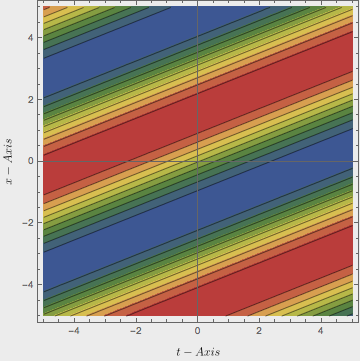
\includegraphics[width=\linewidth]{src/method_of_characteristics/figures/projChar1p1.png}
                      \caption{proj. Char.}
                      \label{fig:projChar1p1}
                    \end{subfigure}%
                    \begin{subfigure}{.6\columnwidth}
                      \centering\tabularnewline
                      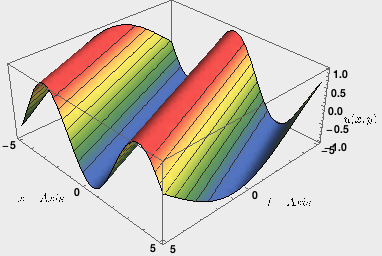
\includegraphics[width=\linewidth]{src/method_of_characteristics/figures/projChar1p2.png}
                      \caption{Solution Surface}
                      \label{fig:projChar1p2}
                    \end{subfigure}
                    \caption{$\psi(s)=\sin(s)$}
                \end{figure}
\end{notebox}

\begin{notebox}[Example 3: \textnormal{$5u_t+2tu_x=0$\hfil $\dot{t}=5,\ \dot{x}=2t,\ \dot{z}=0$}]
                \imp{Initial Conditions}:\hfil $u(x, 0)=\tulm[3]{\sin}(\tulm{x})$\\
                $\Rightarrow$\hfil $\pmat{5 & 2t}\cdot\nabla u=0$\\
                \imp{Parameterisation}:\\
                $\Rightarrow u(\tulm[dotted]{x_s(r)},\tulm[2dotted]{t_s(r)})=\gammac[z]_s(0)=\tc{Brown}{z}_0(s)=u(\tulm[1]{s},\ul{0})=\tulm[3]{\sin}(\tulm{s})$\\
                $\Rightarrow \gammac[x]_s(0)=\tc{Brown}{x}_0(s)=\tulm{s},\
                             \gammac[t]_s(0)=\tc{Brown}{t}_0(s)=\ul{0}$
\end{notebox}
\begin{notebox}[Solution 3]
                \nospacing
                \begin{alignat*}{3}
                    &\gammac[t]_s=5r+c_1(s)                  &  &\xrightarrow{\gammac[t]_s(0)=0} &   & \tulm[6]{\gammac[t]}_s=5\tulm[4]{r}\\
&\dot{\gammac[x]}_s=2\tulm[6]{t}\Rightarrow\gammac[x]_s=5r^2+c_2(s)&    &\xrightarrow{\gammac[x]_s(0)=s}  &  & \gammac[x]_s=5\tulm[4]{r}^2+\tulm[5]{s}      \\
                    &\gammac[z]_s=c(3)_s                 &\     &\xrightarrow{\gammac[z]_s(0)=\sin(s)}&\ & \gammac[z]_s=\sin(\tulm[5]{s})
                \end{alignat*}
                $\Rightarrow$\hfil$ \gammac_s(r)=\pmat{5r & 2r^2+s & \psi(\tulm[5]{s})}$\\
                \imp{Now} we need the inverse transformation $r(x,t),\ s(x,t)$
                $\Rightarrow \gammac[t]_s=5r \Leftrightarrow \tulm[4]{r}=\frac{t}{5}$\qquad
                    $\Rightarrow  \gammac[x]_s=5\tulm[4]{\left(\frac{t}{5}\right)^2}+\tulm[5]{s} \Leftrightarrow
                    \tulm[5]{s}=x-\frac{t^2}{5}$\\
                \imp{Thus}: \ctr{$u(x,t)=\sin(\tulm[5]{x-\frac{t^2}{5}})$}
\end{notebox}
\begin{notebox}[Note]
    $x_s(t)=\frac{1}{5}t^2+s$ are the porjected characteristic curves \cref{fig:projChar2p1} which are constant along $\frac{\diff x}{\diff t}=\frac{2}{5}t$.
                \begin{figure}[H]
                    \centering
                    \begin{subfigure}{.4\columnwidth}
                      \centering
                      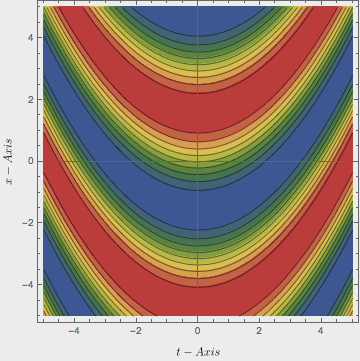
\includegraphics[width=\linewidth]{src/method_of_characteristics/figures/projChar2p1.png}
                      \caption{proj. Char.}
                      \label{fig:projChar2p1}
                    \end{subfigure}%
                    \begin{subfigure}{.6\columnwidth}
                      \centering\tabularnewline
                      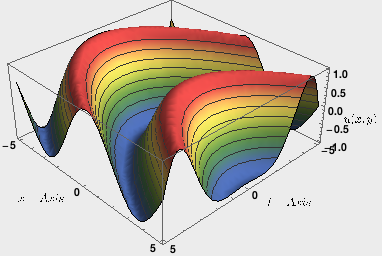
\includegraphics[width=\linewidth]{src/method_of_characteristics/figures/projChar2p2.png}
                      \caption{Solution Surface}
                      \label{fig:projChar2p2}
                    \end{subfigure}
                \end{figure}
\end{notebox}
\begin{sectionbox}[\subsubsection{Case Studie: Burgers Equation}]
\nospacing
    \begin{alignat}{3}
        &u_t+u u_x&=&0 \nonumber\nalign
        &u(x,0)&=&\Phi(x)\label{eq:Burgers Equation}
    \end{alignat}
    \begin{alignat*}{5}
    &\imp{\text{ODEs}}         &\qquad          &\frac{\diff t}{\diff r}=1 &       &\frac{\diff x}{\diff r}=\tulm{u}&          &\frac{\diff u}{\diff r}=0   \nalign
    &\imp{\text{I.C.}}         &\qquad          &\gammac[t](0;s)=0  &\qquad &\gammac[x](0;s)=s           &\qquad   &\gammac[u](0;s)=\Phi(s)
    \end{alignat*}
    \imp{Solution}          \hfil $\gammac[t]_s(r)=r+c_1(s)$\hfil    $\gammac[u]_s(r)=\tulm{c_3(s)}$\\
    $\Rightarrow \frac{\diff x}{\diff r}=\tulm{c_3(s)}$\hfil $\Rightarrow\gammac[x]_s(r)=\tulm{c_3(s)}r+c_2(s)$\\
    \imp{I.C.} \hfil $\gammac[t]_s(r)=r$\hfil $\gammac[u]_s(r)=\tulm{\Phi(\ul{s})}$\hfil $\gammac[x]_s(r)=\tulm{\Phi(s)}r+\ul{s}$\\
    \imp{Invers} \hfil $r=t$\hfil $\ul{s}=x-\phi(s)r=x-\phi(s)t=x-ut$\\
    \imp{Thus}\hfil $u(x,t)=\phi(\ul{x-ut})$\\
    \imp{With} \rd{proj. characteristics}:\hfil $x_{\mc[3]{s}}=\bdra{\phi(\mc[3]{s})}{\normalfont{slope/speed}}t+\mc[3]{s}$
\end{sectionbox}
\begin{sectionbox}[Geometric Interpretation]
    $\phi(\mc[3]{s})$ determines the speed of a characteristic emanating from a given $\mc[3]{s}$:\hfil
    $\begin{cases}
        x=kt+d      \\
        x_{\mc[3]{s}}=\phi(\mc[3]{s})t+\mc[3]{s}  \\
    \end{cases}$
\end{sectionbox}
%%% Local Variables:
%%% mode: latex
%%% TeX-command-extra-options: "-shell-escape"
%%% TeX-master: "../../formulary"
%%% End:
